\documentclass[twocolumn,amsmath,amssymb,showpacs,prl,superscriptaddress,aps]{revtex4-1}

\usepackage{epsfig}
\usepackage{color}
\usepackage{array}
\usepackage{graphicx}
\usepackage{bm}
\usepackage{epstopdf}


\DeclareMathOperator*{\argmin}{argmin}




\begin{document}




\title{Engineering momentum profiles of cold-atom beams}

\author{D~Hudson \surname{Smith}}
\affiliation{Clemson University, Clemson, South Carolina 29634, USA}

\author{Artem~G \surname{Volosniev}}
\affiliation{Institut f{\"u}r Kernphysik, Technische Universit{\"a}t Darmstadt, 64289 Darmstadt, Germany}


\date{\today}

\begin{abstract}
We propose a scheme for engineering fluxes of cold atoms with given momentum profiles. 
In our proposal, the flux is created using a link potential that selects desired momenta 
from the bath. We discuss how to determine the link potential given the required profile 
of a beam, and present a topical application, in which the beam is used 
to study Bose polarons. 
\end{abstract}


\maketitle



{\it Introduction. --} In systems of cold atoms the typical energies are so 
low that usually only a few quantities (e.g., the scattering length and the three-body parameter) 
determine physics~\cite{braaten2006, bloch2008}. 
When these parameters are known the outcomes of measurements can be predicted. 
Ultracold beams with a given momentum might be very useful for determining these parameters. 
For example, the effective mass of a Fermi or Bose `polaron'~\cite{zwierlein2009,hu2016,arlt2016}
can be obtained by studying a beam of particles with a given momentum inside a degenerate gas.
Furthermore, ultracold beams can give new 
insight into the systems where non-universal energy-dependent phenomena have been observed. For instance, it can help 
to understand the temperature (energy) dependence of the three-body parameter~\cite{naidon2011, huang2015, wacker2018}.


In this Letter, we propose an approach for engineering beams of cold atoms. 
Our proposal is illustrated in Fig.~\ref{fig:Figure1}: The particles in a reservoir scatter off the link potential with 
some desired transmission coefficient, $T_0(k)$. The function $T_0(k)$ allows only particles with a given momentum to 
tunnel through the barrier into the `flux region'. In spirit, our scheme is similar to a quantum switch device 
(`transistor')~\cite{zoller2004, marchukov2016}, where the flux of particles from the `source' is affected by changing the properties of the `gate'.
However, the present proposal in addition to completely switching off the flux, allows one to engineer the momentum profile of the flux.




To confirm that the flux has been created one can use a single-atom momentum resolution to check the momentum profile of the flux~\cite{jochim2018}. 




%%%%%%%%%%%%%%%%%%%%%%%%%%%%%%%%%%%%%%%%%%%%%%%%%%%%%%%%%%%%%%%%%%%%%%%%%%%%%%%%%%%%%%%%%%%%%%%%%%%%%%%%%%%%%%%%%%%%%%%
\begin{figure}
\centerline{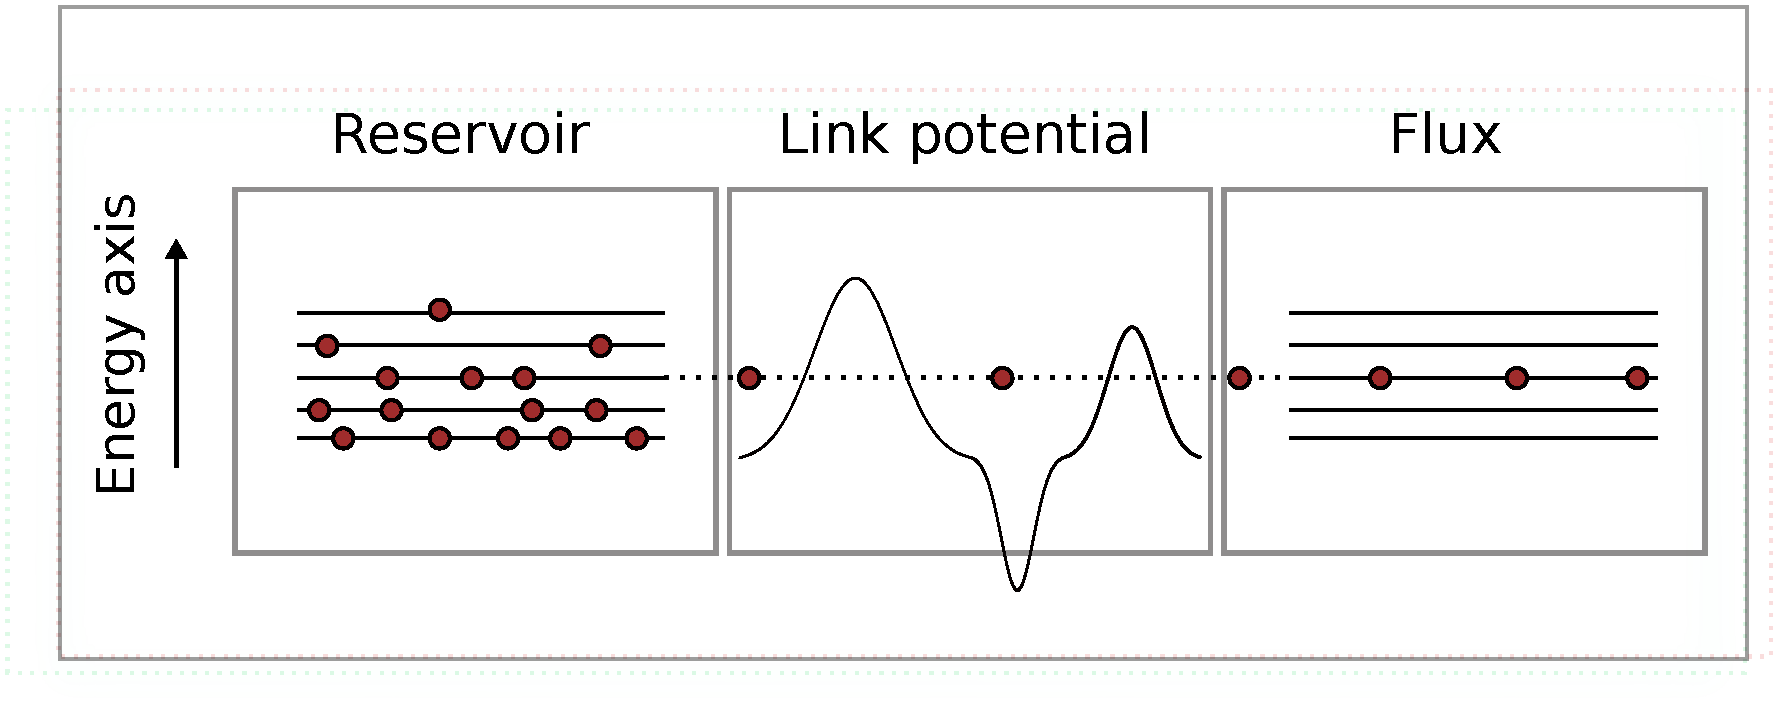
\includegraphics[scale=0.3]{figure1new.pdf}}
\caption{An illustration of the proposal: The reservoir that contains particles of various momenta is connected to the external potential. The design of this potential
allows only particles with desired momenta to tunnel into the flux region.
  }
\label{fig:Figure1}
\end{figure}
%%%%%%%%%%%%%%%%%%%%%%%%%%%%%%%%%%%%%%%%%%%%%%%%%%%%%%%%%%%%%%%%%%%%%%%%%%%%%%%%%%%%%%%%%%%%%%%%%%%%%%%%%%%%%%%%%%%%%%%



\section{Design}

\subsection{Physical System}
Describe the system. The system has three parts: Two reservoirs and a link between them; see Figure 1a. One reservoir is made of a non-interacting (for simplicity) gas of particles at temperature $T$. We call these particles probes or $A$. The reservoir is connected to the link. The link is a potential that acts only on particles $A$ (for simplicity). The second reservoir is made of interacting particles $B$. These particles make a system of interest, which we would like to analyze. 

\subsection{Procedure for Finding a Link Potential}\label{sec:procedure_link}
We find an appropriate link potential $V_0(x) \equiv V(x,\bm{\theta}^*)$ by performing a global search over a family of possible potentials $V(x,\bm{\theta})$ for the parameters $\bm{\theta}^*$ that reduce the $k$-integrated squared error between the desired transmission-momentum profile $T_0(k)$ and the actual profile $T_{\bm\theta}(k)$ determined by a sample potential $V(x, \bm{\theta})$. Concretely, we minimize the cost
\begin{equation}\label{eq:cost1}
  J_{\bm{\theta}} = \sum_kw_k\left|T_0(k) - T_{\mathbf{\theta}}(k)\right|^2,
\end{equation}
where the $k$-integral has been approximated (up to a constant factor) by a sum over a discrete set of momentum values, and $w_k$ is the weight given to momentum $k$. The weights are chosen to emphasize regions of $k$ during the minimization. For instance, when trying to create a ``comb'' potential that forbids transmission for all $k$ except in the neighborhood of a chosen value $k_0$, then it would be appropriate to increase the weights in the region of $k_0$. We find that results are sensitive to the choice of $w_k$, and some trial and error was required to get acceptable potentials. 

With the goal of discovering experimentally viable solutions, we parameterize the family of link potentials $V(x, \bm{\theta})$, as a sum of $N$ Gaussian potentials each of the form
\begin{equation}\label{eq:V-param}
V_i(x; A_i, \mu_i, \sigma_i) = \frac{A_i}{\sqrt{2\pi\sigma_i^2}}\exp\left[{-\frac{(x-\mu_i)^2}{2\sigma_i^2}}\right],
\end{equation}
While minimizing Eq.~\eqref{eq:cost1}, we enforce the parameter constraints listed in Table \ref{tab:constraints}. In addition to these explicit constraints on the parameters, we enforce an implicit constraint by requiring that the link potential should not extend beyond the region of potential support $x\in[-x_0,x_0]$. To accomplish this, we minimize the augmented cost
\begin{equation}\label{eq:cost2}
  J_{\bm{\theta}}^{\mathrm{aug}} = J_{\bm{\theta}} + \alpha \sum_i^N\int\limits_{|x|>x_0}dx\,|V_i(x; A_i,\mu_i,\sigma_i)|^2,
\end{equation}
where $\alpha$ is a tuning parameter chosen to make the added term of a similar order to $J_{\mathbf{\theta}}$ in the scenario that the potential extends outside the support region. Beyond this, we find that results are not very sensitive to the choice of $\alpha$ probably due to the very short tails of the Gaussian potentials. The integral in Eq.~\eqref{eq:cost2} evaluates to the complementary error function. The full form is given in the suppl.~material. 

For a choice of $\bm{\theta}$ (and hence $V(x;\bm{\theta})$), we solve for $T_{\bm{\theta}}(k)$ by integrating Schr{\"o}dinger's equation across the region of the potential and calculating the ratio of the transmitted to the incident flux. In order to do this efficiently, we approximate the integral as a banded linear system of equations solvable in $O(M)$ time where $M$ is the number of $x$-steps. Using these techniques we are able to evaluate the transmission coefficient x thousand times per second on a 7th generation Intel Core i7 processor under the conditions used in our tests. 

 We minimize $J_{\bm{\theta}}^{\mathrm{aug}}$ for $\bm{\theta}^*$ using the global optimization routine called Differential Evolution (DE) \cite{original DE paper}. This evolutionary-based search algorithm is suitable given the non-convex (multiple local minima) nature of the optimization problem. Despite its simplicity, DE does a good job of balancing exploration of the space of link potentials against the need to efficiently learn from each sample with little tuning of the model settings. Emperically, we found DE to perform much better than several other approaches including random search, Nelder-Mead, and Simulated Annealing \cite{Tests performed using mathematica}.

\begin{table}[t]
  \renewcommand*{\arraystretch}{1.4}
  \begin{tabular}{m{3cm}|m{5.5cm}}
    Constraints & Experimental Rationale \\
    \hline\hline
    $\sum_{i=1}^{N}\mu_i = 0$ & The cost function has a continuous degeneracy associated with overall translations of the link potential. \\
    \hline
    $\sigma_{\mathrm{min}} \leq \sigma_j \leq \sigma_{\mathrm{max}} $ & Laser beam widths fall between a minimum and maximum value.\\
    \hline
    $A_{\mathrm{min}} \leq |A_j| \leq A_{\mathrm{max}}$ & Laser amplitudes fall between a minimum and maximum value.
  \end{tabular}
  \caption{The explicit constraints on the potential parameters and the rationale for each constraint. The values of $\sigma_{\mathrm{min}}$, $\sigma_{\mathrm{max}}$, $A_{\mathrm{min}}$, and $A_{\mathrm{max}}$ must be determined from the experimental context.}
  \label{tab:constraints}
\end{table}

Figure \ref{fig:method_examples} demonstrates the application of the procedure described above to three scenarios: the comb potential, evaporative cooling, and anti-evaporative cooling. Each figure shows the resulting link potential $V_0(x)$ along with the target and actual momentum-transmission profiles. 

{\it Figure 2: Examples of a few profiles that can be created: comb, evaporative, anti-evaporative etc. In the insets are the corresponding potentials.}

{\it Application. --} Consider a flux through a degenerate 
one-dimensional Bose gas. If the current is low then the system 
can be described using the concept of the polaron -- an impurity dressed by low-energy excitations 
of the environment~\cite{landau1948}. Let us briefly describe the properties of this quasiparticle
within an extension to the mean-field theory developed in Ref.~\cite{volosniev2017}
for a zero momentum of the impurity~\footnote{See the Supplementary Material}; see also~\cite{kain2016, parisi2017,grusdt2017, pastukhov2017}. 
According to this theory the lowest energy state of a system with a fixed value of momentum, $P$, 
is a combination of two solitons which makes a dissipationless defect in the Bose gas, which we call the polaron. The corresponding energy 
is given by $E\simeq E_B+\epsilon+P^2/(2m_{\mathrm{eff}})$, where $E_B$ is the energy of the gas without an impurity, 
$\epsilon$ is the self-energy of the polaron, and $m_{\mathrm{eff}}$ is its effective mass. The polaron solution is steady only 
for $P<P_c$, where $P_c$ defines the momentum above which the propagation flux produces grey solitons. 
Note that quantum fluctuations will lead to some finite dissipation~\cite{astrakharchik2004,sykes2009} even for $P<P_c$, however
we do no consider this effect in the present study.

Ultracold beams can be used to study the properties of Bose polarons. For example, to measure the effective 
mass one can prepare the flux of particles $B$ in the hyperfine state that does not 
interact with the Bose gas. Then the particles $B$ can be transferred into a hyperfine state that strongly interacts with the gas.
This transfer is possible only if one deposits the energy that compensates for the interaction effects; see Fig.~\ref{fig:Figure3}{\bf a)}. 
There is a non-zero overlap between a free particle and the polaron state; see~\cite{volosniev2017} for $P=0$.
Therefore, by looking at the radio-frequency responce (e.g., the transferred fraction) at different momenta, the effective mass of the polaron can be extracted. 
This idea is similar to a recent experiment in a three-dimensional Fermi polaron~\cite{zaccanti2017}. However,
in our case the initial momentum is known, and therefore not only the effective mass but also the limits of applicability 
of the polaron model can be determined, in particular, the critical momentum above which there are no steady solutions.
In Fig.~\ref{fig:Figure3}{\bf b)} we present this momentum for heavy impurities (for which our theory works best), relevant 
for mixtures of cold atoms with large mass imbalance, e.g., Li-Yb~\cite{takahashi2018}.
For weak interactions ($g\to 0$) the critical momentum is determined by the speed of sound, $c$, in accordance with the Landau criterion.
For strong interactions ($g\to \infty$) the critical momentum goes to zero as $1/g$.  
In this limit the critical momentum is determined by the time needed to exchange two strongly interacting particles. 
 


%%%%%%%%%%%%%%%%%%%%%%%%%%%%%%%%%%%%%%%%%%%%%%%%%%%%%%%%%%%%%%%%%%%%%%%%%%%%%%%%%%%%%%%%%%%%%%%%%%%%%%%%%%%%%%%%%%%%%%%
\begin{figure}
\centerline{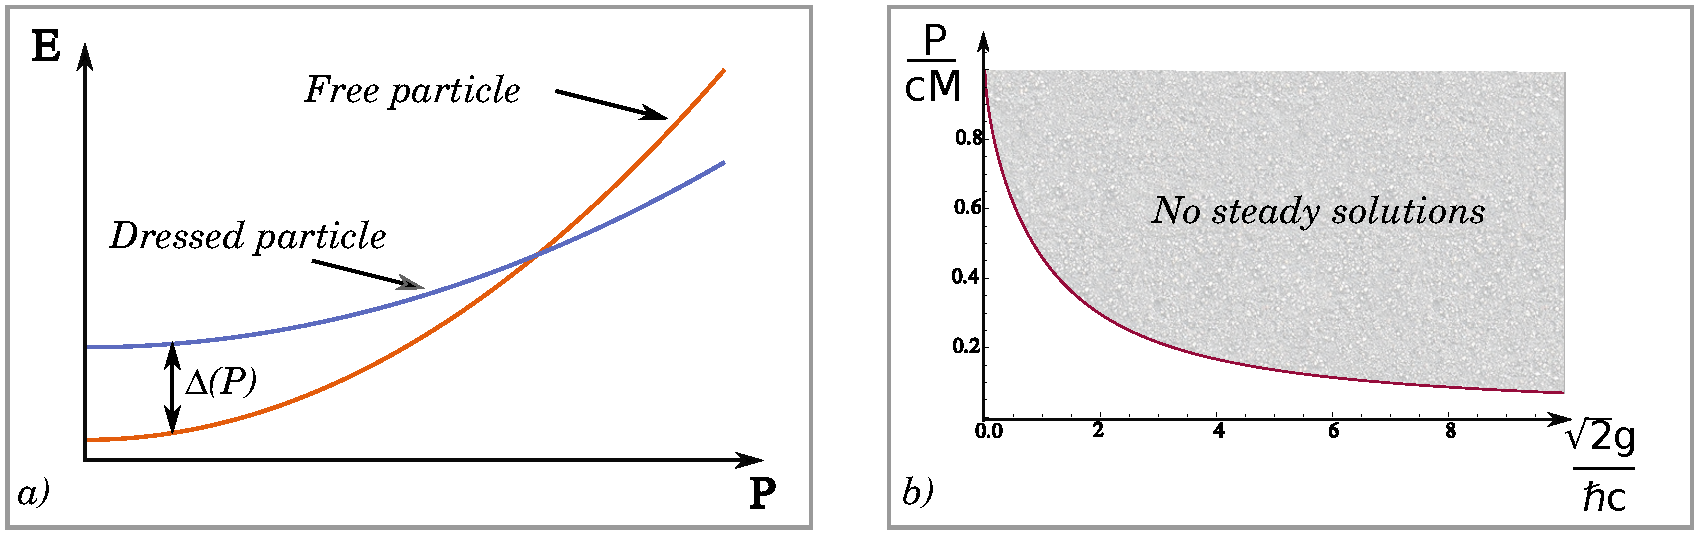
\includegraphics[scale=0.3]{figure3.pdf}}
\caption{Panel {\bf a)} shows schematically the energies of a free particle and a Bose polaron --
a particle in a degenerate Bose gas. The possibility to create particles of a given momenta 
will allow one to establish the effective mass of the polaron
and the limits of applicability of the polaron model by measuring the energy difference, $\Delta(p)$, using the radio-frequency spectroscopy.
Note that quasiparticle properties should be absent for high momenta. For one spatial dimension, a typical momentum scale can be estimated  by considering the existence of steady solutions 
of a suitable non-linear Schr{\"o}dinger equation; see the text for details. Panel {\bf b)} 
shows the results for a heavy impurity of mass $M$; $c$ is the speed of sound
and $g$ is the boson-impurity interaction strength.
  }
\label{fig:Figure3}
\end{figure}
%%%%%%%%%%%%%%%%%%%%%%%%%%%%%%%%%%%%%%%%%%%%%%%%%%%%%%%%%%%%%%%%%%%%%%%%%%%%%%%%%%%%%%%%%%%%%%%%%%%%%%%%%%%%%%%%%%%%%%%



{\it Summary. --}  We have shown how to create beams of particles to probe systems of cold atoms. 
As an application of our proposal we have used the one-dimensional Bose polaron problem. The same concept
can be used to study two-, three- and mixed-dimensional systems. Other interesting applications. 







\begin{acknowledgments}
We thank Georg Bruun for referring to~\cite{zaccanti2017}.
A.~G.~V. gratefully acknowledges the support of the Humboldt Foundation.
\end{acknowledgments}

\widetext

\section{Supplementary Material}

\section{Polaron}

To model one impurity atom that moves through a one-dimensional environment made of $N$ cold bosonic atoms, we employ the following Hamiltonian
\begin{equation}
H=-\frac{\hbar^2}{2m}\sum_{i=1}^N\frac{\partial^2}{\partial x_i^2}-\frac{\hbar^2}{2M}\frac{\partial^2}{\partial y^2}+\lambda \sum_{i>j=1}^N\delta(x_i-x_j)+g \sum_{i=1}^N \delta(x_i-y),
\end{equation}
where $M$ is the mass of the impurity atom, and $m$ is the mass of a bosonic particle. The position of the impurity is $y$, bosons are at the coordinates $\{x_i\}$. 
We assume that the realistic boson-boson and boson-impurity interactions are well-described by the zero-range potentials of strengths $\lambda$ and $g$ respectively. 
The reservoir by assumption is large, such that the dynamics can be described by the thermodynamic limit $N\to \infty$ with a given density $\rho$.
To approach this limit, the periodic boundary conditions are used: The particles move in a ring of the circumference $L$, such that $0<x_i<L$ and $0<y<L$.
We are interested in the limit $N(L)\to \infty$ with $\rho=\frac{N}{L}$.


For $c=0$ the eigenstates can be written as $e^{2\pi i \frac{n_1x_1+\ldots+n_N x_N+my}{L}}$, where $n_1,\ldots,n_N$ and $m$ are arbitrary integrers. 
For $c>0$ this basis set can be used to expand an eigenfunction of the Hamiltonian, $\Psi=\sum_{\{n_j\},m} a_{\{n_j\},m}e^{2\pi i \frac{\sum n_jx_j+my}{L}}$. 
Because all interactions are pairwise, 
the total (angular) momentum of the system must be conserved, and we write it as ${\cal P}=\frac{2\pi\hbar}{L}\left(\sum_{j} n_j+m\right)$.
A conserved quantity (${\cal P}$) allows us to exclude one variable from the consideration. 
We write the function $\Psi$ as $\Psi=e^{i \frac{{\cal P} y}{\hbar}}\sum_{\{n_j\},m} a_{\{n_j\},m}e^{2\pi i \frac{\sum n_jz_j}{L}}\equiv e^{i \frac{{\cal P} y}{\hbar}} \psi(z_1,...,z_N)$ 
with $z_i=L\theta(y-x_i)+x_i-y$, where $\theta(x)$ is the Heaviside step function, i.e., 
$\theta(x>0) = 1$ and zero otherwise. The variables $z_i$ are defined such that $0\leq z_i \leq L$ and the impurity is placed at $z=0$ ($z=L$). Now if we insert this 
function into the Schr{\"o}dinger equation, $H\Psi=E\Psi$, we obtain the following equation for $\psi(0<z_i<L)$
\begin{equation}
-\frac{\hbar^2}{2m}\sum_i\frac{\partial^2 \psi}{\partial z_i^2}-\frac{\hbar^2}{2M}\left(\sum_{i}\frac{\partial }{\partial z_i}\right)^2\psi
+ i \frac{\hbar {\cal P}}{M}\sum_{i}\frac{\partial \psi}{\partial z_i}+\lambda \sum_{i>j}\delta(z_i-z_j)\psi=\left(E-\frac{{\cal P}^2}{2M}\right)\psi,
\end{equation}
which must be supplemented with the boundary conditions:
\begin{equation}
\psi(z_i=0)=\psi(z_i=L); \qquad \frac{\partial \psi}{\partial z_i}\bigg|^{z_i=0^+}_{z_i=L^-}= \frac{2 g \kappa}{\hbar^2} \psi(z_i=0),
\end{equation}
where $\kappa=mM/(m+M)$ is the reduced mass.

By assumption the bosons interact weakly, such that the ansatz $\psi=\prod_i \Phi(z_i)$ can be used to approximate the system. 
To minimize the expectation value of the Hamiltonian the function $\Phi(z)$ must satisfy the following non-linear Schr{\"o}dinger equation
\begin{equation}
-\frac{\hbar^2}{2\kappa}\frac{\partial^2\Phi}{\partial z^2}+i\frac{\hbar {\cal P}}{M}\frac{\partial \Phi}{\partial z}
-i \frac{\hbar^2 (N-1) A}{M} \frac{\partial\Phi}{\partial z} + \lambda (N-1)|\Phi|^2\Phi=\mu \Phi,
\end{equation}
where $A=-i\int \Phi(x)^*\frac{\partial}{\partial x}\Phi(x)\mathrm{d}x$ defines the momentum of a boson, and $\mu$ is the Lagrange multiplier. 
We rewrite this equation as
\begin{equation}
-\frac{\partial^2\Phi}{\partial z^2}+i v \frac{\partial \Phi}{\partial z} + \tilde \lambda (N-1)|\Phi|^2\Phi=\tilde\mu\Phi,
\label{eq:GPE_resc}
\end{equation}
where $\tilde\mu=\frac{2 \kappa \mu}{\hbar^2}$, $\tilde \lambda =\frac{2 \kappa \lambda}{\hbar^2}$, and 
$v\equiv \frac{2 \kappa P}{M \hbar}$, where $P={\cal P}-\hbar A(N-1)$ defines the momentum of the impurity in the thermodynamic limit;
note that because $A$ is determined by $P$, there is a unique value of ${\cal P}$ for a given $P_I$.
The corresponding boundary conditions read
\begin{equation}
\Phi(z=0)=\Phi(z=L); \qquad \frac{\partial \Phi}{\partial z}\bigg|^{z=0^+}_{z=L^-}= \tilde g \Phi(0),
\end{equation}
where $\tilde g= \frac{2\kappa g}{\hbar^2}$. The non-linear equation~(\ref{eq:GPE_resc}) 
has an analytic steady solution~\cite{hakim1997}, which determines the properties 
of the polaron in our problem. Let us first consider the non-interacting case $\lambda=0$. In this case the solution for $v>0$ is~\cite{tsuzuki1971, ishikawa1980}
\begin{equation}
\Phi=\sqrt{\frac{\tilde \mu}{\tilde \lambda (N-1)}}\left(1-\beta \mathrm{sech}^2\left[\sqrt{\frac{\tilde\mu\beta}{2}}(z+z_0)\right]\right)^{\frac{1}{2}}e^{i\phi(z)},
\label{eq:Phi_c0}
\end{equation}
\begin{equation}
\phi(z)=-\pi\theta(z+z_0)+\mathrm{arctan}\left(\frac{\sqrt{\frac{2 v^2}{\tilde \mu}\beta}}{\mathrm{exp}\left[\sqrt{2\tilde \mu\beta}(z+z_0)\right]-2\beta+1}\right),
\label{eq:phi_c0}
\end{equation}
where  $\beta=1- v^2/(2\tilde \mu)$, and $z_0$ is some parameter that determines the origin. It is worthwhile noting that the solution for $v<0$ is $\Phi^*$. 
The solution from Eqs.~(\ref{eq:Phi_c0}) and~(\ref{eq:phi_c0}) is plotted in Fig.~\ref{fig:Fig1}; 
for simplicity it is plotted in the interval $-L/2<z<L/2$, the region $0<z<L$ easily follows. By combining the solutions with $\pm z_0$ 
one can construct a steady solution with a singularity at $z=0$~\cite{hakim1997}. Therefore, the `polaron' in this model is a superposition of two moving solitons. 
In other words, the impurity creates a topological defect, which leads to a dissipationless propagation. 

%%%%%%%%%%%%%%%%%%%%%%%%%%%%%%%%%%%%%%%%%%%%%%%%%%%%%%%%%%%%%%%%%%%%%%%%%%%%%%%%%%%%%%%%%%%%%%%%%%%%%%%%%%%%%%%%%%%%%%%
\begin{figure}
\centerline{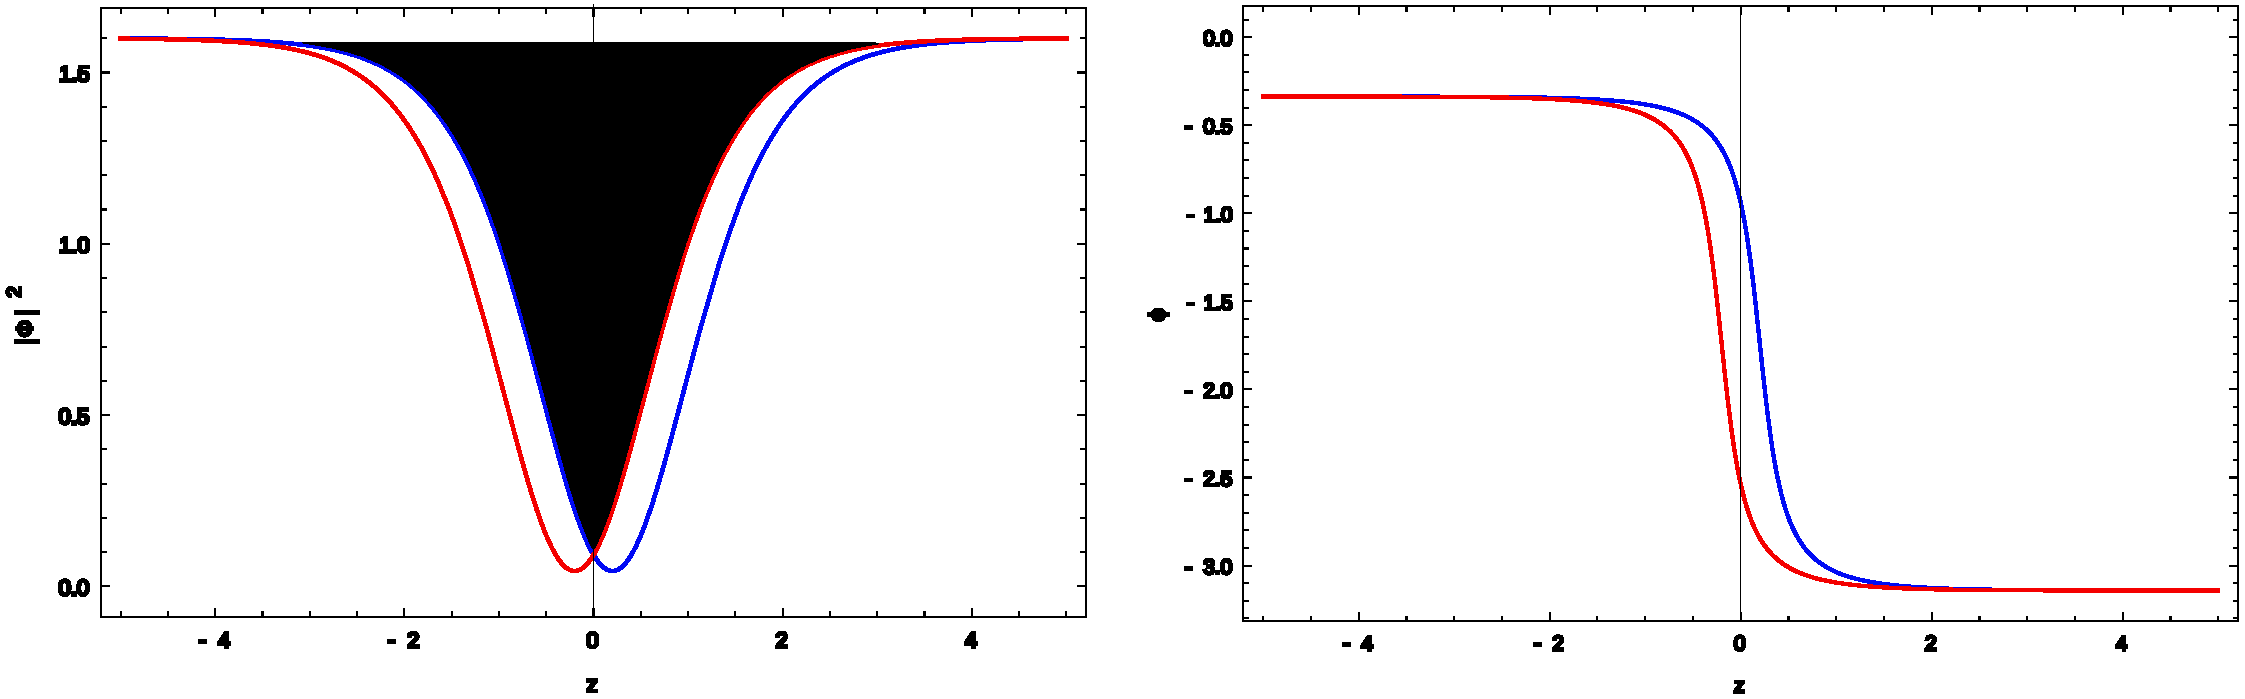
\includegraphics[scale=0.45]{figure1appendix.pdf}}
\caption{Panel {\bf a)}: The density, $|\Phi|^2 \tilde \lambda (N-1)$, of the Bose gas for two different parameters $z_0$: $z_0=0.2$ (left red curve), $z_0=-0.2$ (right blue curve), 
assuming that $\tilde \mu=1.6, v=0.3$ (everything is in units where $\rho=1$). 
Note that the minimum of the density is at $-z_0$. The shaded area is a combination of the two solutions with the singularity at $z=0$. Panel {\bf b)}: The phase, $\phi$, of the Bose gas for the densities from {\bf a)}.}
\label{fig:Fig1}
\end{figure}
%%%%%%%%%%%%%%%%%%%%%%%%%%%%%%%%%%%%%%%%%%%%%%%%%%%%%%%%%%%%%%%%%%%%%%%%%%%%%%%%%%%%%%%%%%%%%%%%%%%%%%%%%%%%%%%%%%%%%%%

We write the wave function for the polaron as
\begin{equation}
\Phi=\sqrt{\frac{\tilde \mu}{\tilde \lambda (N-1)}}\left(1-\beta \mathrm{sech}^2\left[\sqrt{\frac{\tilde\mu\beta}{2}}(z\pm z_0)\right]\right)^{\frac{1}{2}}e^{i\phi(z)},
\end{equation}
with 
\begin{equation}
\phi(z)=\delta \phi \theta(-z)+\mathrm{arctan}\left(\frac{\sqrt{\frac{2 v^2}{\tilde \mu}\beta}}{\mathrm{exp}\left[\sqrt{2\tilde \mu\beta}(z\pm z_0)\right]-2\beta+1}\right),
\label{eq:phase_soliton}
\end{equation}
where $z_0>0$ is discussed below, the parameter $\delta \phi$ is not important for the further derivations, it reassures that the phase is a continuous function;
the plus sign in $\pm$ corresponds to $z>0$ and the minus sign to $z<0$. This function is illustrated in Fig.~\ref{fig:Fig1}. 
The density has a non-analytic derivative at $z=0$. The phase is a continuous function at $z=0$ (its derivative is also continuous).
Note that the wave function is not periodic (see Eq.~(\ref{eq:phase_soliton})). This non-periodicity is not important 
for our discussion, because we are interested in the behavior of the bosons close to the impurity. It suggests that a grey soliton
must be formed upon a change of interaction parameters to take care of the phase slip.

The parameter $\tilde \mu$ is found from the normalization condition $\int \Phi^2=1$. For $N\to\infty$, we obtain
\begin{equation}
\tilde \mu=\gamma \rho^2 \frac{N-1}{N}\left(1-2\sqrt{2\beta_0} \frac{ (\mathrm{tanh}(d)-1)}{\sqrt{\gamma}N}\right),
\end{equation}
where $\gamma=\tilde \lambda /\rho$, $\rho=N/L$, $\beta_0=1-v^2/(2\gamma \rho^2)$, and $d=\sqrt{\frac{\gamma \beta_0}{2}}\rho z_0$.
The equation to determine $z_0$ is found by using the boundary conditions at $z=\{0,L\}$
\begin{equation}
\frac{\tilde g}{\rho \sqrt{2\gamma}}=\frac{\beta_0^{\frac{3}{2}}\tanh(d)}{-\beta_0+\cosh^2(d)}.
\label{eq:c_v}
\end{equation}
This equation is cubic (in $\tanh(d)$), hence, the solutions can be found in a closed form.
There are three solutions. However, only two will lead to the acceptable values of $z_0$. 
We will refer to these steady solutions as the `polaron' and the `polaron-soliton' pair, because in the limit $g\to 0$ the former 
corresponds to the ground state, and the latter to a gray soliton. 
The `polaron-soliton' pair is expected to be unstable (small perturbations will lead to 
a decay of this steady solution~\cite{hakim1997}),
therefore, we do not consider it. The solutions merge for $z_m$ 
\begin{equation}
\tanh^2\left(\sqrt{\frac{\gamma \beta_0}{2}}\rho z_m\right)=\frac{\sqrt{1+\frac{4v^2}{\gamma \rho^2}}-(1+\frac{v^2}{\gamma \rho^2})}{2\beta_0},
\label{eq:z_m}
\end{equation}
which is derived by taking a derivative of Eq.~(\ref{eq:c_v}) with respect to $z_0$ and equating the resulting expression to zero -- this determines 
the maximum value of $g$ for which (for a fixed $\beta_0$) there is a steady solution.
Equations~(\ref{eq:c_v}) and (\ref{eq:z_m}) give the equation for the critical value of $v_c$:
\begin{equation}
\frac{\tilde g}{\rho\sqrt{\gamma}}=\frac{3-\sqrt{1+\frac{4v_c^2}{\gamma \rho^2}}}{-1+\sqrt{1+\frac{4v_c^2}{\gamma \rho^2}}}\sqrt{\sqrt{1+\frac{4v_c^2}{\gamma \rho}}-1-\frac{v_c^2}{\gamma\rho^2}}.
\end{equation}
For $v>v_c$ (see Fig. 1 of the main text) there is no steady solutions.


Now we can calculate the energy of the polaron in the thermodynamic limit
\begin{equation}
{\cal E}\equiv \lim_{N\to\infty, \frac{N}{L}\to \rho}\left[E(c,P)-E(c=0,P=0)\right],
\end{equation}
where
\begin{equation}
E(c,P) = \frac{P^2}{2M} + \mu N-\frac{\hbar^2 A^2 N(N-1)}{2M}-gN(N-1)\int_{0}^{L/2}|\Phi|^4\mathrm{d}z.
\end{equation}
Using these expressions we derive 
\begin{equation}
{\cal E}=\frac{P_I^2}{2M}+\frac{\hbar^2\rho}{2\kappa}\frac{\sqrt{2 \tilde g \rho \beta}}{3}\left[4 b + (-4b+\beta\mathrm{sech}^2(d))\tanh(d)\right]+\frac{\hbar P_I}{M}\lim_{N\to\infty} A N,
\end{equation}
where $b=1+\frac{v^2}{4\tilde g\rho}=1+\frac{\kappa P_I^2}{2M^2 g\rho}$. This energy for $v\to 0$ can be written as 
\begin{equation}
{\cal E}\simeq \epsilon+ \frac{P_I^2}{2m_{\mathrm{\mathrm{eff}}}},
\end{equation}
where $\epsilon$ is the effective energy of the polaron, and $m_{\mathrm{eff}}$ is the effective mass.





\subsection{Cost Function}\label{sec:cost_function}

\begin{equation}
  J'_{\mathbf{\theta}} = J_{\mathbf{\theta}} + \alpha J_{\mathrm{boundary}},
\end{equation}
where $\alpha>0$ is the weight given to cost incurred for having the potential extend outside the support region of the potential.



\bibliographystyle{apsrev4-1}
\bibliography{bib}

 \end{document}


